\PassOptionsToPackage{dvipsnames}{xcolor}

\documentclass[10pt]{article} % For LaTeX2e
\usepackage[preprint]{tmlr}
% If accepted, instead use the following line for the camera-ready submission:
%\usepackage[accepted]{tmlr}
% To de-anonymize and remove mentions to TMLR (for example for posting to preprint servers), instead use the following:
%\usepackage[preprint]{tmlr}

\usepackage{amssymb,amsmath,amsthm,mathtools}
\usepackage{hyperref}
\usepackage{url}
\usepackage{upquote}
\usepackage{booktabs}

\usepackage{microtype}
\UseMicrotypeSet[protrusion]{basicmath} % disable protrusion for tt fonts

\usepackage{xcolor}

\usepackage{hyperref}
\hypersetup{
  colorlinks = true,
  breaklinks = true,
  linkcolor  = black,
  filecolor  = MidnightBlue,
  citecolor  = MidnightBlue,
  urlcolor   = MidnightBlue
}

\usepackage{cleveref}

% Optional math commands from https://github.com/goodfeli/dlbook_notation.
\input{math_commands.tex}
% operators
\DeclareMathOperator*{\argmax}{arg\,max}
\DeclareMathOperator*{\argmin}{arg\,min}
\DeclareMathOperator{\E}{E}
\DeclareMathOperator{\var}{Var}
\DeclareMathOperator{\cov}{Cov}
\DeclareMathOperator{\tr}{tr}
\DeclareMathOperator{\diag}{diag}
\DeclareMathOperator{\range}{range}
\DeclareMathOperator{\nullspace}{null}
\DeclareMathOperator{\rank}{rank}
\DeclareMathOperator{\card}{card}
\DeclareMathOperator{\sign}{sign}
\DeclareMathOperator{\st}{S}
\DeclareMathOperator{\normal}{Normal}
\DeclareMathOperator{\fnormal}{FoldedNormal}
\DeclareMathOperator{\bernoulli}{Bernoulli}
\DeclareMathOperator{\erf}{erf}
\DeclareMathOperator{\mse}{MSE}
\DeclareMathOperator{\risk}{R}
% \DeclareMathOperator{\I}{I}
% \DeclareMathOperator{\T}{}

\renewcommand{\vec}{\symbf}
\newcommand{\mat}{\symbf}
\newcommand*\du{\mathop{}\!\mathrm{d}}
\newcommand{\T}{\intercal}
\newcommand{\ones}{\symbf{1}}
\newcommand{\ind}[1]{\operatorname{I}_{#1}}

% \newcommand{\todojl}[1]{\todo[color=green!40]{#1}}

% \newcommand{\mv}[1]{{\boldsymbol{\mathrm{#1}}}}



\title{Formatting Instructions for TMLR \\Journal Submissions}

% Authors must not appear in the submitted version. They should be hidden
% as long as the tmlr package is used without the [accepted] or [preprint] options.
% Non-anonymous submissions will be rejected without review.

\author{%
  \name Johan Larsson \email johan.larsson@stat.lu.se\\
  \addr Deparment of Statistics\\Lund University
  \AND
  \name Jonas Wallin \email jonas.wallin@stat.lu.se\\
  \addr Department of Statistics\\Lund University
}

% The \author macro works with any number of authors. Use \AND 
% to separate the names and addresses of multiple authors.

\newcommand{\fix}{\marginpar{FIX}}
\newcommand{\new}{\marginpar{NEW}}

\def\month{MM}  % Insert correct month for camera-ready version
\def\year{YYYY} % Insert correct year for camera-ready version
\def\openreview{\url{https://openreview.net/forum?id=XXXX}} % Insert correct link to OpenReview for camera-ready version

\begin{document}

\maketitle

\begin{abstract}
  The abstract paragraph should be indented 1/2~inch on both left and
  right-hand margins. Use 10~point type, with a vertical spacing of 11~points.
  The word \textbf{\large Abstract} must be centered, in bold, and in point size 12. Two
  line spaces precede the abstract. The abstract must be limited to one
  paragraph.
\end{abstract}

\section{Introduction}

When the data you want to model is high-dimensional, that is, the number of features \(p\) exceed the number of observations \(n\), it is impossible to apply classical statistical models such as standard linear regression since the design matrix \(\mat X\) is no longer of full rank. A common remedy to this problem is to \emph{regularize} the model by adding a term to the objective function that punishes models with large coefficients (\(\vec\beta\)). If we let \(h(\vec\beta; \mat X, \vec y)\) be the original objective function---which when minimized improves the model's fit to the data (\(\mat X, \vec y\))---then
\[
  f(\beta_0, \vec\beta; \mat X, \vec y) = h(\beta_0, \vec\beta; \mat X, \vec y) + g(\vec\beta)
\]
is a composite function within which we have added a penalty term \(g(\vec\beta)\).
In contrast to \(h\), this penalty depends only on the coefficients (\(\vec{\beta}s\)).
The intercept, \(\beta_0\), is not typically penalized.

Some of the most common penalties are the \(\ell_1\) and \(\ell_2\) penalties, that is \(g(\vec\beta) = \lVert \vec\beta \rVert_1\) or \(g(\vec\beta) = \lVert \vec\beta \rVert_2^2/2\)\footnote{Division by two in this case is used only for convenience.}, which, if \(h\) is the standard ordinary least-squares objective, represent lasso~\citep{tibshirani1996,santosa1986,donoho1994} and ridge (Tikhonov) regression respectively.
Other common penalities include SLOPE~\citep{bogdan2013,bogdan2015}, MCP~\citep{zhang2010}, hinge loss (used in support vector machines~\citep{cortes1995}) and SCAD~\citep{fan2001}.
Many of these penalities---indeed all of the previously mentioned ones---shrink coefficients in proportion to their sizes.

% TODO: Maybe say something about ℓ₀ (best subset) regularization

The issue with this type of shrinkage is that it is typically sensitive to the scales and locations of the features in \(\mat X\).
A common remedy is to \emph{normalize} the features before fitting the model by translating and dividing each column by respective translation and scaling factors.
For some problems, such factors may arise naturally from knowledge of the problem at hand.
A researcher may for instance have collected data on coordinates within a limited area and know that the coordinates are measured in meters.
Often, however, these scaling and location factors must be estimated from data.
The most popular choices for this type of scaling are based only on the marginal distributions of the features.
Some types of normalization, such as that applied in the adaptive lasso\footnote{The adaptive lasso typically uses estimates of the regression coefficients, typically from ordinary-least squares or ridge regression, to scale the features with.}~\citep{zou2006}, however, are based on the conditional distributions of the features and the response.
After fitting the model, the estimated coefficients are then usually returned to their original scale.

Another reason for normalizing the features is to improve the performance and stability of optimization algorithms used to fit the model.
We will not cover this aspect in this paper, but note that it is an important one.

In most sources and discussions on regularized methods, normalization is typically treated as a preprocessing step---separate from modeling. As we will show in this paper, however, the type of normalization used can have a critical effect on the estimated model, sometimes leading to entirely different conclusions with regard to feature importance as well as predictive performance. As a first example of this, consider \Cref{fig:realdata-paths}, which displays the lasso paths for three real data sets and three different types of normalization. Each panel shows the union of the first five predictors picked by either type of normalization. As we can see, the choice of normalization can have a significant impact on the estimated model. In the case of the \texttt{leukemia} data set, for instance, the models are starkly different with respect to both the identities of the features selected as well as their signs and magnitudes.

\begin{figure}[bpt]
  \centering
  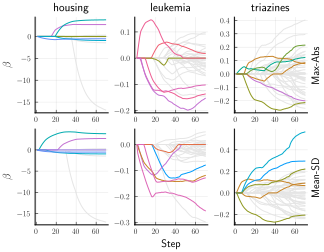
\includegraphics[]{plots/realdata_paths.pdf}
  \caption{%
    A display over the first predictors selected by the lasso for each type of normalization. Each panel shows the union of the first five predictors picked by either type of normalization.
  }
  \label{fig:realdata-paths}
\end{figure}

In addition, discussions on the choice of normalization are often focused on computational aspects and data storage requirements, rather than on the statistical properties of the choice of normalization. In our paper, we will argue that normalization should rather we considered as an integral part of the model. And that it for instance is unreasonable to base the choice of normalization on the type of data storage, which implicitly encodes the belief that a data set stored as a sparse matrix is somehow fundamentally different from a data set stored as a dense matrix.

\section{Preliminaries}

Throughout this paper, we assume that the data is generated from a linear model, \(y_i =
\beta_0^* + \vec x_i^\T \vec\beta^* + \varepsilon_i\) for \(i \in [n]\) where \([n] =
\{1,2,\dots,n\}\) and we use \(\beta_0^*\) and \(\vec\beta^*\) to denote the true intercept
and coefficients, respectively, and \(\varepsilon_i\) to denote measurement noise. \(\mat
X\) is the \(n \times p\) design matrix with features \(\vec x_j\) and \(\vec y\) the \(n
\times 1\) response vector. Furthermore, we use \(\hat\beta_0\) and \(\hat{\vec{\beta}}\)
to denote our estimates of the intercept and coefficients. Unless we state otherwise, we
assume \(\mat{X}\), \(\beta_0^*\), and \(\vec{\beta}^*\) to be fixed.%

There is much ambiguity regarding key terms in the field of normalization. \emph{Scaling},
\emph{standardization}, and \emph{normalization} are for instance used interchangeably
throughout the literature. Here, we define \emph{normalization} as the process of centering
and scaling the feature matrix, which we now formalize.

\begin{definition}[Normalization]
  \label{def:normalization}
  % Let \(\mat S\) be the \emph{scaling matrix}, which is a \(p \times p\) diagonal matrix with entries \(s_1, s_2, \dots, s_p\). Let \(\mat C\) be the \emph{centering matrix}, which is an \(n \times p\) matrix with each row equal to \([c_1, c_2, c_n]^\T\). Then the \emph{normalized design matrix} \(\tilde{\mat X}\) is defined as \(\tilde{\mat X} = (\mat X - \mat C)\mat S^{-1}\).
  Let \(\tilde{\mat X}\) be the normalized feature matrix, with elements \(\tilde{x}_{ij} =
  (x_{ij} - c_{j})/s_j,\) where \(x_{ij}\) is an element of the (unnormalized) feature matrix
  \(\mat{X}\) and \(c_j\) and \(s_j\) are the \emph{centering} and \emph{scaling} factors
  respectively.
\end{definition}

Some authors refer to the procedure in \Cref{def:normalization} as \emph{standardization},
but here we define standardization only as the case when centering with the mean and
scaling with the (uncorrected) standard deviation.

\subsection{Types of Normalization}

There are many different strategies for normalizing the design matrix. We list a few common
choices in \Cref{tab:normalization-types}. Standardization is perhaps the most popular type
of normalization, at least in the field of statistics. One of its benefits is that it
simplifies certain aspects of fitting the model, such as fitting the intercept. The
downside of standardization is that it involves centering by the mean, which destroys
sparsity. This is not a problem when \(\bm{X}\) is stored as a dense matrix; but when the
data is sparse, it may increase memory use and processing time.

% TODO: move to appendix?
\begin{table}[hbt]
  \centering
  \caption{
    Common ways to normalize a matrix of features using centering and scaling
    factors \(c_j\) and \(s_j\), respectively. Note that \(\bar{x}_j =
    n^{-1}\sum_{i=1}^n x_{ij}\).
  }
  \label{tab:normalization-types}
  \vskip 0.15in
  \small
  \begin{tabular}{lll}
    \toprule
    Normalization            & \(c_{j}\)          & \(s_j\)                                                   \\
    \midrule
    Standardization          & \(\bar{x}_j\)      & \(\sqrt{\frac{1}{n}\sum_{i=1}^n (x_{ij} - \bar{x}_j)^2}\) \\
    \addlinespace
    Max--Abs                 & 0                  & \(\max_i|x_{ij}|\)                                        \\
    \addlinespace
    Min--Max                 & \(\min_i(x_{ij})\) & \(\max_i(x_{ij}) - \min_i(x_{ij})\)                       \\
    \addlinespace
    \(\ell_1\)-Normalization & 0 or \(\bar{x}_j\) & \(\lVert \vec{x}_j\rVert_1\)                              \\
    \addlinespace
    Adaptive Lasso           & 0                  & \(\beta_j^\text{OLS}\)                                    \\
    \bottomrule
  \end{tabular}
\end{table}

When the data is sparse, a common alternative to standardization is to scale features by
their maximum absolute values (max--abs normalization). This method has no impact on binary
data\footnote{Except in the extreme case when all values are 0.} and therefore retains
sparsity. For other types of data, it scales the features to take values in the range
\([-1, 1]\). Since the scaling is determined by a single value for each feature, the method
is naturally sensitive to outliers. For many types of data, such as normally distributed
data, it is also often the case that the sample maximum depends on sample size, which often
makes use of the method problematic~(\Cref{thm:maxabs-gev}~(\Cref{sec:additional-theory})

% TODO: should we study l1-normalization more?
Min-max normalization scales the data to lie in \([0, 1]\). As with the max--abs method,
min-max normalization retains sparsity and also shares its sensitivity to outliers and
sample size. Unlike max--abs scaling, however, min--max scaling is not sensitive to the
\emph{location} of the data, only its \emph{spread}. In \(\ell_1\)-normalization, each
feature is scaled with its sum of absolute value. The method is common in signal
processing. A special case of normalization is the adaptive lasso~\citep{zou2006}, which is
a two-step procedure. First we fit a model such as ordinary least-squares (OLS) or ridge
regression. Then we use the estimated coefficients to scale the features and refit.

\subsection{The Lasso, Ridge Regression, and the Elastic Net}

Let \((\hat{\beta}_0^{(n)}, \hat{\vec{\beta}}^{(n)})\) be a solution to the problem in
\Cref{eq:elastic-net}. Expanding \(f\) in \Cref{eq:elastic-net}, we have
\[
  \begin{aligned}
     & \frac{1}{2}\left( \vec y^\T \vec y - 2(\tilde{\mat{X}}\vec{\beta} + \beta_0)^\T\vec{y} + (\tilde{\mat{X}}\vec{\beta} + \beta_0)^\T(\tilde{\mat{X}}\vec{\beta} + \beta_0)\right) \\
     & + \lambda_1 \lVert \vec\beta \rVert_1 + \frac{\lambda_2}{2}\lVert \vec \beta \rVert_2^2.
  \end{aligned}
\]
Taking the subdifferential with respect to \(\vec{\beta}\) and \(\beta_0\), the KKT
stationarity condition yields the following system of equations:
\begin{equation}
  \label{eq:kkt-elasticnet}
  \begin{cases}
    \tilde{\mat{X}}^\T(\tilde{\mat{X}}\vec{\beta} + \beta_0 - \vec{y}) + \lambda_1 g + \lambda_2 \vec\beta \ni \vec{0}, \\
    n \beta_0 + (\tilde{\mat{X}}\vec{\beta})^\T \vec{1} - \vec{y}^\T \vec{1} = 0,
  \end{cases}
\end{equation}
where \(g\) is a subgradient of the \(\ell_1\) norm that has elements \(g_i\) such that
\[
  g_i \in
  \begin{cases}
    \{\sign{\beta_i}\} & \text{if } \beta_i \neq 0, \\
    [-1, 1]            & \text{otherwise}.
  \end{cases}
\]

\subsection{Weighted Penalization}%
\label{sec:weighted-elasticnet}

One alternative to normalization, which will be of particular interest in the case of the
elastic net, is to weight the coefficients in the penalty term---and instead of minimizing
\Cref{eq:elastic-net} minimize the following objective:
\[
  \begin{multlined}
    \tilde{f}(\beta_0, \vec{\beta}, \mat{X}, \vec{y}, \lambda_1, \lambda_2) =\\
    \frac{1}{2} \lVert \vec{y} - \beta_0 - \mat{X}\vec{\beta}\rVert_2^2 + \lambda_1 \sum_{j=1}^p u_j |\beta_j| + \frac{\lambda_2}{2} \sum_{j=1}^p v_j \beta_j^2,
  \end{multlined}
\]
with \(\vec{u}\) and \(\vec{v}\) being \(p\)-length vectors of positive scaling factors. We
call this the \emph{weighted elastic net}, which is equivalent to the original form when
\(u_j = s_j\) and \(v_j = s_j^2\), which can be seen by substituting \(\beta_js_j =
\tilde{\beta}_j\) in \Cref{eq:elastic-net} and solving for \(\tilde{\vec{\beta}}\).

\subsection{Orthogonal Features}

If the features of the normalized design matrix are orthogonal, that is,
\(\tilde{\mat{X}}^\intercal \tilde{\mat{X}} = \diag\left(\tilde{\vec{x}}_1^\T
\tilde{\vec{x}}_1, \dots, \tilde{\vec{x}}_p^\intercal \tilde{\vec{x}}_p\right) \), then
\Cref{eq:kkt-elasticnet} can be decomposed into a set of \(p + 1\) conditions:
%
\[
  \begin{cases}
    \tilde{\vec{x}}_j^\T (\tilde{\vec{x}}_j \beta_j + \ones \beta_0 - \vec{y}) + \lambda_2 \beta_j + \lambda_1 g \ni 0, & j \in [p], \\
    n \beta_0 + (\tilde{\mat{X}}\vec{\beta})^\T \vec{1} -  \vec{y}^\T \ones = 0.
  \end{cases}
\]
%
The inclusion of the intercept ensures that the locations (means) of the features do not
affect the solution (except for the intercept itself). We will therefore from now on assume
that the features are mean-centered so that \(c_j = \bar{\vec{x}}_j\) for all \(j\) and
therefore \(\tilde{\vec{x}}_j^\T \ones = 0\). A solution to the system of equations is then
given by the following set of equations~\citep{donoho1994}:
%
\begin{equation*}
  \label{eq:orthogonal-solution-normalized}
  \hat{\beta}^{(n)}_j = \frac{\st_{\lambda_1}\left(\tilde{\vec{x}}_j^\T \vec{y}\right)}{\tilde{\vec{x}}_j^\T \tilde{\vec{x}}_j + \lambda_2},
  \qquad
  \hat{\beta}_0^{(n)} = \frac{\vec{y}^\T \ones}{n},
\end{equation*}
%
where \(\st_\lambda(z) = \sign(z) \max(|z| - \lambda, 0)\) is the soft-thresholding
operator.

\subsection{Rescaling Regression Coefficients}

Normalization changes the optimization problem and its solution, the coefficients, which
will now be on the scale of the normalized features. But we are interested in
\(\hat{\vec{\beta}}\): the coefficients on the scale of the original problem. To obtain
these, we transform the coefficients from the normalized poblem, \(\hat\beta^{(n)}_j\),
back via
%
\begin{equation}
  \label{eq:orthogonal-solution}
  \hat\beta_j = \frac{\hat\beta^{(n)}_j}{s_j} \quad\text{for}\quad j = 1,2,\dots,p.
\end{equation}
%
There is a similar transformation for the intercept but we omit here since we are not
interested in it. Note that this rescaling is not needed in the weighted elastic
net~(\Cref{sec:weighted-elasticnet}), since the estimated coefficients are kept on the same
scale as the original (non-normalized) data.

\section{Bias-Variance Tradeoffs in Data with Binary Features}

Now, assume that \(\mat{X}\) and \(\vec{\beta}\) are fixed and that \(\vec{y} = \mat{X}\vec{\beta} + \vec{\varepsilon}\), where \(\varepsilon_i\) is identically and independently distributed noise with mean zero and finite variance \(\sigma_\varepsilon^2\). We are interested in the expected value of \Cref{eq:orthogonal-solution}. Let \(Z = \tilde{\vec{x}}_j^\T \vec{y} = \tilde{\vec{x}}_j^\T(\mat{X}\vec{\beta} + \vec{\varepsilon})\) and \(d_j = s_j\left(\tilde{\vec{x}}_j^\T \tilde{\vec{x}}_j + \lambda_2\right)\) so that \(\hat{\beta}_j = \st_{\lambda_1}(Z)/d_j\). We start by focusing on the numerator, since the denominator, \(d_j\), is fixed. First observe that
\[
  \E Z = \mu = \E \left( \tilde{\vec{x}}_j^\T (\vec{x}_j\beta_j + \vec{\varepsilon}) \right)  = \tilde{\vec{x}}_j^\T\vec{x}_j \beta_j.
\]
And for the variance, we have
\[
  \var Z = \sigma^2 = \var\left(\tilde{\vec{x}}_j ^\T \vec{\varepsilon}\right) = \sigma_\varepsilon^2 \lVert \tilde{\vec{x}}_j\rVert_2^2 .
\]

The expected value of the soft-thresholding estimator is
\begin{align}
  \label{eq:st-expected-value}
  \E \st_\lambda(Z) & = \int_{-\infty}^\infty \st_\lambda(z) f_Z(z) \du z                                                   \nonumber \\
                    & = \int_{-\infty}^\infty \ind{|z| > \lambda} (z -\sign(z)\lambda) f_Z(z) \du z                         \nonumber \\
                    & = \int_{-\infty}^{-\lambda}(z + \lambda)f_Z(z) \du z + \int_{\lambda}^\infty (z - \lambda)f_Z(z) \du z.
\end{align}
And then the bias of \(\hat\beta_j\) with respect to the true coefficient \(\beta_j^*\) is
\begin{equation}
  \label{eq:betahat-bias}
  \E \hat\beta_j - \beta_j^* = \frac{1}{d_j}\E \st_\lambda(Z) - \beta^*_j.
\end{equation}

Finally, we note that the variance of the soft-thresholding estimator is
\begin{equation}
  \label{eq:st-variance}
  \var {S_\lambda(Z)} = \int_{-\infty}^{-\lambda}(z + \lambda)^2f_Z(z) \du z + \int_{\lambda}^\infty (z - \lambda)^2 f_Z(z) \du z - \left(\E \st_\lambda(Z)\right)^2
\end{equation}
and that the variance of the elastic net estimator is therefore
\begin{equation}
  \label{eq:betahat-variance}
  \var \hat\beta_j = \frac{1}{d_j^2} \var \st_\lambda(Z).
\end{equation}

% \subsection{Normally Distributed Noise}

Next, we add the additional assumption that \(\vec{\varepsilon}\) is normally distributed. Then
\[
  Z \sim \normal\left(\tilde{\vec{x}}_j^\T\vec{x}_j \beta_j, \sigma_\varepsilon^2 \lVert \tilde{\vec{x}}_j\rVert_2^2 \right).
\]
Let \(\theta = -\mu -\lambda_1 \) and \(\gamma = \mu - \lambda_1\). Then the expected value of soft-thresholding of \(Z\) is
\begin{align}
  \E \st_{\lambda_1}(Z) & = \int_{-\infty}^\frac{\theta}{\sigma} (\sigma u - \theta) \pdf(u) \du u + \int_{-\frac{\gamma}{\sigma}}^\infty (\sigma u + \gamma) \pdf(u) \du u                                               \nonumber                      \\
                        & = -\theta \cdf\left(\frac{\theta}{\sigma}\right) - \sigma \pdf\left(\frac{\theta}{\sigma}\right) + \gamma \cdf\left(\frac{\gamma}{\sigma}\right) + \sigma \pdf\left(\frac{\gamma}{\sigma}\right) \label{eq:mean-centered-eval}
\end{align}
where \(\pdf(u)\) and \(\cdf(u)\) are the probability density and cumulative distribution functions of the standard normal distribution, respectively.

Next, we consider what the variance of the elastic net estimator looks like.
Starting with the first term on the left-hand side of \Cref{eq:st-variance}, we have
\begin{multline}
  \label{eq:mc-var-part1}
  \int_{-\infty}^{-\lambda_1}(z+ \lambda_1)^2 f_Z(z) \du z = \sigma^2 \int_{-\infty}^{\frac{\theta}{\sigma}} y^2 \pdf(y) \du y + 2 \theta \sigma \int_{-\infty}^{\frac{\theta}{\sigma}} y \pdf(y) \du y + \theta^2 \int_{-\infty}^{\frac{\theta}{\sigma}} \pdf(y) \du y \\
  = \frac{\sigma^2}{2} \left( \erf\left(\frac{\theta}{\sigma\sqrt{2}}\right) - \frac{\theta}{\sigma}\sqrt{\frac{2}{\pi}} \exp\left(-\frac{\theta^2}{2\sigma^2}\right) + 1 \right) + 2 \theta \sigma \pdf \left(\frac{\theta}{\sigma}\right) + \theta^2 \cdf\left(\frac{\theta}{\sigma}\right).
\end{multline}
Similar computations for the second term on the left-hand side of \Cref{eq:st-variance} yield
\begin{multline}
  \label{eq:mc-var-part2}
  \int_{\lambda_1}^{\infty}(z - \lambda_1)^2 f_Z(z) \du z \\
  = \frac{\sigma^2}{2} \left( \erf\left(\frac{\gamma}{\sigma\sqrt{2}}\right) - \frac{\gamma}{\sigma}\sqrt{\frac{2}{\pi}} \exp\left(-\frac{\gamma^2}{2\sigma^2}\right) + 1 \right) + 2 \gamma \sigma \pdf \left(\frac{\gamma}{\sigma}\right) + \gamma^2 \cdf\left(\frac{\gamma}{\sigma}\right).
\end{multline}
Plugging \Cref{eq:mean-centered-eval,eq:mc-var-part1,eq:mc-var-part2} into \Cref{eq:betahat-variance} yields the variance of the estimator. Consequently, we can also compute the mean-squared error via the bias-variance decomposition
\begin{equation}
  \label{eq:betahat-mse}
  \mse (\hat\beta_j, \beta^*_j) = \var\hat\beta_j + \left(\E \hat\beta_j - \beta^*_j\right)^2.
\end{equation}

% \subsubsection{Binary Features}

Our results have so far covered the general case where we have made no assumptions on \(\mat{X}\), except for being non-random. But our main focus in this paper
is the case when \(\vec{x_j}\) is a binary feature with class balance \(q\), that is, \(x_{ij} \in \{0, 1\}\) for all \(i\) and \(\sum_{i=1}^n x_{ij} = nq\).
In this case, we observe that
\[
  \begin{aligned}
    \tilde{\vec{x}}_j^\T \tilde{\vec{x}}_j & = \frac{1}{s_j^2}(\vec{x}_j - \ones c_j)^\T (\vec{x}_j - \ones c_j) = \frac{1}{s^2_j}(nq - 2nq^2 + nq^2) = \frac{nq(1-q)}{s^2_j}, \\
    \tilde{\vec{x}}_j^\T \vec{x}_j         & = \frac{1}{s_j}(\vec{x}_j^\T \vec{x}_j - \vec{x}_j^\T \ones c_j) = \frac{nq(1 - q)}{s_j}.
  \end{aligned}
\]
And consequently
\[
  \mu = \frac{\beta^*_j nq(1 - q)}{s_j}, \qquad \sigma^2 = \frac{\sigma_\varepsilon^2nq(1 - q)}{s^2_j}, \qquad d_j = \frac{nq(1 -q)}{s_j}  + \lambda_2 s_j.
\]
We will allow ourselves to abuse notation and overload the definitions of \(\mu\), \(\sigma^2\), and \(d_j\) as functions of \(q\). Then, an expression for the expected value of the elastic net estimate with respect to \(q\) can be obtained by plugging in \(\mu\) and \(\sigma\) into \Cref{eq:mean-centered-eval}.

We are mainly interested in examining the case when \(\vec{x}_j\) is imbalanced and what effect various approaches to normalizing the features
has on the elastic net estimator. In order to study this, we will parameterize the scaling factors \(s_j\) for \(j  \in [p]\) by \(s_j = (q - q^2)^\delta\), \(\delta \geq 0\).
This includes the cases that we are primary interested in, that is,
\begin{itemize}
  \item \(\delta = 0\): no scaling, which includes min--max and max--abs normalization,
  \item \(\delta = 1/2\): standardization, and
  \item \(\delta = 1\): scaling by the variance.
\end{itemize}
Note that the last of these cases does not correspond to a standard type of normalization. But as we will see, it has some interesting properties in the case of binary features.

A natual consequence of the normal distribution of \(Z\) is that the probability of selection in the elastic net problem is given by
\begin{align*}
  \Pr\left(\hat{\beta}_j \neq 0\right) & = \Pr\left(\st_{\lambda_1}(Z) \neq 0\right)                                                                                         \\
                                       & = \Pr\left(Z > \lambda_1\right) + \Pr\left(Z < -\lambda_1\right)                                                                    \\
                                       & = \cdf\left(\frac{\mu - \lambda_1}{\sigma}\right) + \cdf\left(\frac{- \mu -\lambda_1}{\sigma}\right).                               \\
                                       & = \cdf \left( \frac{\beta_j^*n (q-q^2)^{1/2} - \lambda_1(q-q^2)^{\delta - 1/2}}{\sigma_\varepsilon \sqrt{n}}\right)                 \\
                                       & \phantom{={}} + \cdf \left( \frac{-\beta_j^*n (q-q^2)^{1/2} - \lambda_1(q-q^2)^{\delta - 1/2}}{\sigma_\varepsilon \sqrt{n}}\right).
\end{align*}

Letting \(\theta = -\mu - \lambda_1 \) and \(\gamma = \mu - \lambda_1\), we can express the probability of selection in the limit as \(q \rightarrow 1^+\) as
\[
  \lim_{q \rightarrow 1^+} \Pr(\hat{\beta}_j \neq 0) =
  \begin{cases}
    0                                                                & \text{if } 0 \leq \delta < \frac{1}{2}, \\
    2\cdf\left(-\frac{\lambda_1}{\sigma_\varepsilon \sqrt{n}}\right) & \text{if } \delta = \frac{1}{2},        \\
    1                                                                & \text{if } \delta > \frac{1}{2}.
  \end{cases}
\]

\begin{figure}[htpb]
  \centering
  \includegraphics[]{plots/selection_probability.pdf}
  \caption{%
    Probability of selection in the elastic net problem given a measurement noise level \(\sigma_\varepsilon\), a regularization parameter \(\lambda_1\), and a class balance \(q\). The scaling factor is parameterized by \(s_j = (q - q^2)^\delta\), \(\delta \geq 0\). The dotted line represents the asymptotic limit for the standardization case, \(\delta = 1/2\). }
  \label{fig:selection-probability}
\end{figure}

In \Cref{thm:classbalance-bias}, we show what the
bias is under mean-centering and scaling with \(s_j = (q - q^2)^\delta\), \(\delta \geq 0\).

\begin{theorem}
  \label{thm:classbalance-bias}
  If \(\vec{x}_j\) is a binary feature with class balance \(q \in (0, 1)\), \(\lambda_1 \in (0,\infty)\), \(\lambda_2 \in [0,\infty)\), \(\sigma_\varepsilon > 0\), and \(s_j = (q - q^2)^{\delta}\), \(\delta \geq 0\)  then
  \[
    \lim_{q \rightarrow 1^+} \E \hat{\beta}_j =
    \begin{cases}
      0                                                                                                  & \text{if } 0 \leq \delta < \frac{1}{2}, \\
      \frac{2n \beta_j^*}{n + \lambda_2} \cdf\left(-\frac{\lambda_1}{\sigma_\varepsilon \sqrt{n}}\right) & \text{if } \delta = \frac{1}{2},        \\
      \beta^*_j                                                                                          & \text{if } \delta \geq 1.
    \end{cases}
  \]
\end{theorem}

\begin{corollary}[Bias in Ridge Regression]
  \label{cor:ridge-bias}
  Asume the conditions of \Cref{thm:classbalance-bias} but that \(\lambda_1 = 0\). Then
  \[
    \lim_{q \rightarrow 1^+} \E \hat{\beta}_j =
    \begin{cases}
      0                                         & \text{if } 0 \leq \delta < 1/2, \\
      \frac{\beta_j^*}{1 + \frac{\lambda_2}{n}} & \text{if } \delta = 1/2,        \\
      0                                         & \text{if } \delta > 1/2.
    \end{cases}
  \]
\end{corollary}

\Cref{thm:classbalance-bias} shows that the bias of the elastic net estimator when \(0 \leq \delta < 1/2\), which includes to the case of min--max and max--abs normalization (no scaling), approaches
\(-\beta_j^*\) as \(q \rightarrow 1^+\). When \(\delta = 1/2\) (standardization), the lasso estimate does not vanish completely. Instead, it approaches the
true coefficient scaled by the probability that a standard normal variable is smaller than \(\beta_j^*\sqrt{n}\sigma_\varepsilon^{-1}\). For \(\delta \geq 1\), the
estimate is unbiased asymptotically. The last fact may seem somewhat counterintuitive but is a consequence of the variance of the distribution of the estimator exploding as \(q \rightarrow 1^+\).

\begin{theorem}
  \label{thm:classbalance-variance}
  If \(\vec{x}_j\) is a binary feature with class balance \(q \in (0, 1)\) and \(\lambda_1,\lambda_2 \in (0,\infty)\), \(\sigma_\varepsilon > 0\), and \(s_j = (q - q^2)^{\delta}\), \(\delta \geq 0\), then
  \[
    \lim_{q \rightarrow 1^+} \var \hat{\beta}_j =
    \begin{cases}
      0      & \text{if } 0 \leq \delta < \frac{1}{2}, \\
      \infty & \text{if } \delta \geq \frac{1}{2}.
    \end{cases}
  \]
\end{theorem}

\begin{corollary}[Variance in Ridge Regression]
  \label{cor:ridge-variance}
  Assume the conditions of \Cref{thm:classbalance-variance} but that \(\lambda_1 = 0\). Then
  \[
    \lim_{q \rightarrow 1^+} \var \hat{\beta}_j =
    \begin{cases}
      0                                          & \text{if } 0 \leq \delta < 1/4, \\
      \frac{\sigma_\varepsilon^2 n}{\lambda_2^2} & \text{if } \delta = 1/4,        \\
      \infty                                     & \text{if } \delta > 1/4.
    \end{cases}
  \]
\end{corollary}

\begin{figure}[htpb]
  \centering
  \includegraphics[]{plots/bias-var-onedim.pdf}
  \caption{%
    Bias, variance, and mean-squared error for a one-dimensional lasso problem.
    Note that \(\delta = 0\) corresponds to the case of no scaling, \(\delta = 1/2\) corresponds
    to standardization, and \(\delta = 1\) corresponds to scaling with the variance. The dotted
    lines represent the asymptotic bias of the lasso estimator in the case of \(\delta = 1/2\).
  }
  \label{fig:bias-var-onedim-lasso}
\end{figure}

\subsection{Multiple Predictors}

\begin{figure}[htpb]
  \centering
  \includegraphics[]{plots/beta-bias-multidim.pdf}
  \caption{%
    Mean-squared-error, false discovery rate (FDR), and power for a lasso problem with
    \(k = 10\) true signals (nonzero \(\beta_j^*\)), varying \(p\), and \(q \in [0.5, 0.9, 0.99]\). The noise level is set at \(\sigma_\varepsilon = 1\).
  }
  \label{fig:mse-fdr-power-multidim}
\end{figure}

\section{Mixed Data}
\label{sec:mixed-data}

A natural follow-up topic to the discussion in the previous section is to consider the case where the features are of mixed type, that is, some are continuous and some are binary.
To be able to compare normalization methods with respect to these cases, we need to construct problems in which the coefficients of the continuous and binary features are, in some sense, comparable.
In this section, we will discuss what it means for a continuous and binary feature to have \emph{comparable} effects and how the choice of normalization needs to be adapted to ensure that our penalized estimates respect this notion of comparability.

In this pape, we will focus on normally distrubted continuous features. We acknowledge that this is a limiting choice, but leave it to future papers to approach this issue for other types of distributions.

We will assume that the effect of a change in the binary variable (going from 0 to 1) corresponds to a difference of two standard deviations in the normally distributed variable. We base this choice on the reasoning by \citet{gelman2008}. In other words, if the regression coefficient of the binary variable is \(\beta^*_1\), then the effect corresponding to a normally distributed random variable is equivalent if \(\beta^*_2 = (2\sigma)^{-1} \beta_1^*\).

\begin{example}
  If \(\vec{x}_2\) is sampled from \(\normal(\mu, 2)\), then the effects of \(\vec{x}_1\) and \(\vec{x}_2\) are equivalent if \(\beta_1^* = 1\) and \(\beta_2^* = 0.25\).
\end{example}

Our particular choice of two standard deviations is not critical for our results, which hold for any other choice, as long it is linear with respect to the standard deviation of the normally distributed variable.

On the other hand, we also assume that the effects are equivalent irrespective of the class balance of the binary feature. In other words, we say that two binary features \(\vec{x}_1\) and \(\vec{x}_3\) have equivalent effects as long as \(\beta_1^* = \beta_3^*\), even if the values in \(\vec{x}_1\) are spread evenly between zeros and ones and those of \(\vec{x}_3\) are all zeros except for one. We will see that this is a fundamental assumption upon which our results hinge entirely.

We will cover cases where the continuous feature is not normally distributed on a case-by-case basis as we proceed through the paper.



\section{Experiments}%
\label{sec:experiments}

In the following sections we present the results of our experiments. For all simulated data
we generate our response vector according to \(\vec{y} = \mat{X}\vec{\beta}^* +
\vec{\varepsilon},\) with \(\vec{\varepsilon} \sim \normal(\vec{0}, \sigma_\varepsilon^2
\mat{I})\). We consider two types of features: binary (quasi-Bernoulli) and quasi-normal
features. To generate binary vectors, we sample \(\ceil{nq_j}\) indexes uniformly at random
without replacement from \([n]\) and set the corresponding elements to one and the
remaining ones to zero. To generate quasi-normal features, we generate a linear sequence
\(\vec{w}\) with \(n\) values from \(10^{-4}\) to \(1 - 10^{-4}\), set \(x_{ij} =
\cdf^{-1}(w_i)\), and then shuffle the elements of \(\vec{x}_j\) uniformly at random.

We use a coordinate descent solver to optimize our models, which we have based on the
algorithm outlined by \citet{friedman2010}. All experiments were coded using the Julia
programming language~\citep{bezanson2017} and the code is available at
\url{https://github.com/jolars/normreg}. All simulated experiments were run for 50
iterations and, unless stated otherwise, are presented as means $\pm$ one standard
deviation (using bars or ribbons).

\subsection{Normalization in the Lasso and Ridge Regression}%
\label{sec:experiments-lassoridge}

In this section we consider fitting the lasso and ridge regression to normalized data sets.
To normalize the data, we use standardize all quasi-normal features. For binary features,
we center by mean and scale by \(s_j \propto (q_j-q_j^2)^\delta\).
% where \(\delta = 0\)
% corresponds to no scaling, \(\delta = 1/2\) to standardization, and \(\delta = 1\) to
% variance scaling.

\subsubsection{Variability and Bias in Estimates}\label{sec:experiments-varbias}

In our first experiment, we consider fitting the lasso to a simulated data set with
\(n=500\) observations and \(p = \num{1000}\) features, out of which the first 20 features
correspond to signals, with \(\beta_j^*\) decreasing linearly from 1 to 0.1. We introduce
dependence between the features by copying the first \(\ceil{\rho n/2}\) values from the
first feature to each of the following features. In addition, we set the class balance of
the first 20 features so that it decreases linearly on a log-scale from 0.5 to 0.99. We
estimate the regression coefficients using the lasso, setting \(\lambda_1 = 2
\sigma_\varepsilon \sqrt{2 \log p }\).

The results~(\Cref{fig:binary-decreasing}, and \Cref{fig:binary-decreasing-full} in
\Cref{sec:additional-results-biasvar}) show that class balance has considerable effect,
particularly in the case of no scaling (\(\delta = 0\)), which corroborates our theory from
\Cref{sec:theory-binary-features}. At \(q_j=0.99\), for instance, the estimate
(\(\hat{\beta}_{20}\)) is consistently zero when \(\delta = 0\). For \(\delta=1\), we see
that class imbalance increases the variance of the estimates. What is also clear is that
the variance of the estimates increase with class imbalance and that this effect increases
together with \(\delta\).

\begin{figure}[htpb]
  \centering
  \includegraphics[]{plots/binary_decreasing_small.pdf}
  \caption{%
    Regression coefficients for a lasso problem with binary data where \(n = 500\) and
    \(p = \num{1000}\) with 20 true signals. Here we show only the first 30
    coefficients. See \Cref{sec:experiments-lassoridge} for more information
    on the setup of this experiment.
  }
  \label{fig:binary-decreasing}
\end{figure}

\subsubsection{Predictive Performance}%
\label{sec:experiments-hyperparameter}

Our previous results indicate that the choice of normalization matters also for predictive
performance, and in this section we will examine whether that is the case for three
different data sets: \data{a1a}~\citep{becker1996}, \data{rhee2006}~\citep{rhee2006}, and
\data{w1a}~\citep{platt1998}.\footnote{See \Cref{sec:data-summary} for details about these
  data sets.} We consider performance in terms of normalized mean-squared error~(NMSE) for
lasso and ridge regression across a two-dimensional grid of \(\delta\) and \(\lambda\),
where for \(\delta\) we use a linear sequence from 0 to 1, and for \(\lambda\) a geometric
sequence from \(\lambda_\text{max}\) (the value of \(\lambda\) at which the first feature
enters the model) to \(10^{-2}\lambda_\text{max}\). We split the data into equal training
and validation set splits and for each combination of \(\lambda\) and \(\delta\) fit the
lasso or ridge to the training set.

We present the results for ridge regression in \Cref{fig:hyperopt-contours}, which shows
contour plots of the validation set error. We see that optimal setting of \(\delta\)
differs between the different data sets, suggesting that it might be useful to choose
\(\delta\) by hyperparameter optimization. See
\Cref{fig:hyperopt-contours-full}~(\Cref{sec:predictive-performance-simulated}) for a plot
that includes the lasso as well.

% For
% \data{a1a}, the lasso is generally quite insensitive to the type of normalization, even if
% the optimal value is around 0.2. For ridge regression, lower values of \(\delta\) clearly
% work better. With the \data{w1a} data set, however, the relationship is flipped in the case
% of ridge regression and the optimal value is approximately 0.8. In the case of the lasso
% (for \(\data{w1a}\)), a value around 0.5 is optimal and low values (little scaling) yield
% worse prediction errors. Finally, for \data{rhee2006}, the lasso is again insensitive to
% normalization type. This is not the case for ridge, however, where a value around 0.2 is
% optimal and high values of \(\delta\) yield worse prediction errors.

\begin{figure}[htpb]
  \centering
  \includegraphics[]{plots/hyperopt_surfaces_small.pdf}
  \caption{%
    Contour plots of normalized validation set mean-squared error (NMSE)
    for combinations of \(\delta\) and \(\lambda\) in ridge regression on
    three real data sets. The
    dotted path shows the smallest NMSE as a function of \(\lambda\) and the circles mark
    combinations with the lowest error.
  }
  \label{fig:hyperopt-contours}
\end{figure}

% We would like to point out that there is a dependency between \(\lambda\) and \(\delta\)
% that make it difficult to interpret the relationship between them and the error. This comes
% from the fact that scaling with a smaller value (as in \(\delta = 1\)) increases the sizes
% of the vectors, which means that the level of penalization is relaxed, relatively speaking.

In \Cref{sec:predictive-performance-simulated}, we extend these results with experiments on
simulated data under various class balances and signal-to-noise ratios, again showing that
normalization has an impact on predictive preformance.

\subsubsection{Mixed Data}\label{sec:experiments-mixed-data}

In \Cref{sec:mixed-data} we showed that care needs to be taken when normalizing mixed data.
In our next experiment, we construct a quasi-normal feature with mean zero and standard
deviation 1/2 and a binary feature with varying class balance \(q_j\). We set the
signal-to-noise ratio to 0.5 and use \(n = \num{1000}\). These features are constructed so
that their effects are comparable under the notion of comparability that we introduced in
\Cref{sec:mixed-data} using \(\kappa = 2\). In order to preserve the comparability for the
baseline case when we have perfect class balance, we scale by \(s_j = 2 \times
(1/4)^{1-\delta}(q_j-q_j^2)^\delta\). Finally, we set \(\lambda\) to
\(\lambda_\text{max}/2\) and \(2\lambda_\text{max}\) for lasso and ridge regression
respectively.

The results~(\Cref{fig:lasso-ridge-comparison}) reflect our theoretical results from
\Cref{sec:theory}. In the case of the lasso, we need \(\delta =1\) (variance scaling) to
avoid the effect of class imbalance, whereas for ridge we instead need \(\delta =1/2\)
(standardization). As our theory suggests, this extra scaling mitigates this class-balance
dependency at the cost of added variance.
% Note that we do not see the bias reduction that
% we observed in our theoretical results for high \(q_j\) values and \(\delta \geq 1/2\) in
% \Cref{fig:lasso-ridge-comparison}. This is related to the error term (signal-to-noise
% ratio) and level of \(q_j\). We would need stronger class imbalance and larger error for
% the effect to show up here.

\begin{figure}[htpb]
  \centering
  \includegraphics{plots/mixed_data.pdf}
  \caption{%
    Lasso and ridge estimates for a two-dimensional problem where one feature is a binary
    feature with class balance \(q_j\) (\(\bernoulli(q_j)\)) and the other is quasi-normal
    with standard deviation 1/2, (\(\normal(0, 0.5)\)).
  }
  \label{fig:lasso-ridge-comparison}
\end{figure}

\subsubsection{Interactions}\label{sec:experiments-interactions}

Next, we study the effects of normalization and class balance on interactions in the lasso.
Our example consists of a two-feature problem with an added interaction term given by
\(x_{i3} = x_{i1}x_{i2}\). The first feature is binary with class balance \(q\) and the
second quasi-normal with standard deviation 0.5. We set \(n=1000\), specify \(\lambda_1 =
n/4\). Here, we normalize the binary feature by mean-centering and scaling by \(\kappa (q -
q^2)\), with \(\kappa = 2\). We consider two different strategies for choosing \(s_3\): in
the first strategy, which we call \emph{Strategy 1}, we simply standardize the resulting
interaction feature.
% TODO: make a reference to where this is done
In the second strategy, \emph{Strategy 2} we center with mean and scale with \(s_1s_2\)
(the product of the scales of the binary and normal features).

The results for the case when \(\bm{\beta}^* = \bm{1}\)~(\Cref{fig:interactions}) show that
only strategy 2 estimates the effect of the interaction correctly. Strategy 1, meanwhile,
only selects the correct model if the class balance of the binary feature is close to 1/2
and in general shrinks the coefficient too much. See
\Cref{fig:interactions-full}~(\Cref{sec:additional-experiments-interactions}) for results
on different choices of \(\bm{\beta}^*\).

\begin{figure}[htpb]
  \centering
  \includegraphics[]{plots/interactions-classbalance-small.pdf}
  \caption{%
    Lasso estimates for a problem with a binary feature, a quasi-normal feature, and
    an interaction feature. We have set \(\bm{\beta}^* = \bm{1}\) and use two different normalization strategies where
    Strategy 1 represents standardization and Strategy 2 is mean-centering
    together with scaling by \(s_1 s_2\).
  }
  \label{fig:interactions}
\end{figure}

\subsection{The Weighted Elastic Net}%
\label{sec:experiments-elasticnet}

The weighted elastic net can be used as an alternative to normalization to correct for
class balance bias when \(\lambda_1 > 0\) and \(\lambda_2 >0\). To simplify the
presentation, we parameterize the elastic net as \(\lambda_1 = \alpha \lambda \) and
\(\lambda_2 = (1-\alpha) \lambda\), so that \(\alpha\) controls the balance between the
ridge and lasso. We conduct an experiment with the same setup as in
\Cref{sec:experiments-mixed-data}, but here we use the weighted elastic net instead with
\(\alpha = 0.5\) (See \Cref{sec:additional-experiments-weighted-elnet} for results using
other setting for \(\alpha\)). We use \(n=1000\) and vary \(\omega\), using the weights
\(u_j = v_j = (q_j - q_j^2)^{\omega}\) as we suggested in \Cref{sec:binary-weighting}. Our
results (\Cref{fig:mixed-data-elnet}) show that \(\omega = 1\) leads to seemingly unbiased
estimates.

\begin{figure}[htpb]
  \centering
  \includegraphics{plots/mixed_data_elnet_small.pdf}
  \caption{%
    Weighted elastic net estimates for \(\alpha = 0.5\) for a problem with a binary
    feature with class balance \(q\) (\(\bernoulli(q)\)) and quasi-normal
    with standard deviation 1/2 (\(\normal(0, 0.5)\)). \(\omega\) indicates
    the scaling of the penalty weights.
  }
  \label{fig:mixed-data-elnet}
\end{figure}



% \subsubsection*{Broader Impact Statement}
%
% In this optional section, TMLR encourages authors to discuss possible repercussions of their work,
% notably any potential negative impact that a user of this research should be aware of.
% Authors should consult the TMLR Ethics Guidelines available on the TMLR website
% for guidance on how to approach this subject.

% \subsubsection*{Acknowledgments}
%
% Use unnumbered third level headings for the acknowledgments. All
% acknowledgments, including those to funding agencies, go at the end of the paper.
% Only add this information once your submission is accepted and deanonymized.

\bibliography{normreg}
\bibliographystyle{tmlr}

\appendix

\section{Appendix}

\input{tex/appendix.tex}

\end{document}
